\clearpage
\section{Trade-off analyses}
\label{app:tradeoff-analyses}


\textbf{Stability-plasticity trade-off}

As the model adapts to new data during fine-tuning (plasticity), how well does it retain its previous knowledge (stability)? To study this question, we evaluate the upstream performance of the pretrained models and fine-tuned models using five language understanding and commonsense reasoning benchmarks (\hellaswag{}, \piqa{}, \winogrande{}, \arceasy{}, and \arcchallenge{}) and measure upstream performance using the average accuracy.
We measure stability using the difference in upstream performance between the fine-tuned and pretrained models for a given weight decay value (smaller difference, higher stability) and plasticity using the average downstream performance on the six chain-of-thought reasoning tasks (higher downstream performance, higher plasticity).

We find that while models with higher plasticity also tend to have higher upstream performance after fine-tuning (Figure~\ref{fig:app-plasticity-vs-upstreamacc}), this higher plasticity sometimes comes with a trade-off in stability (Figure~\ref{fig:app-plasticity-vs-stability}).


\begin{figure}[H] 
    \centering
        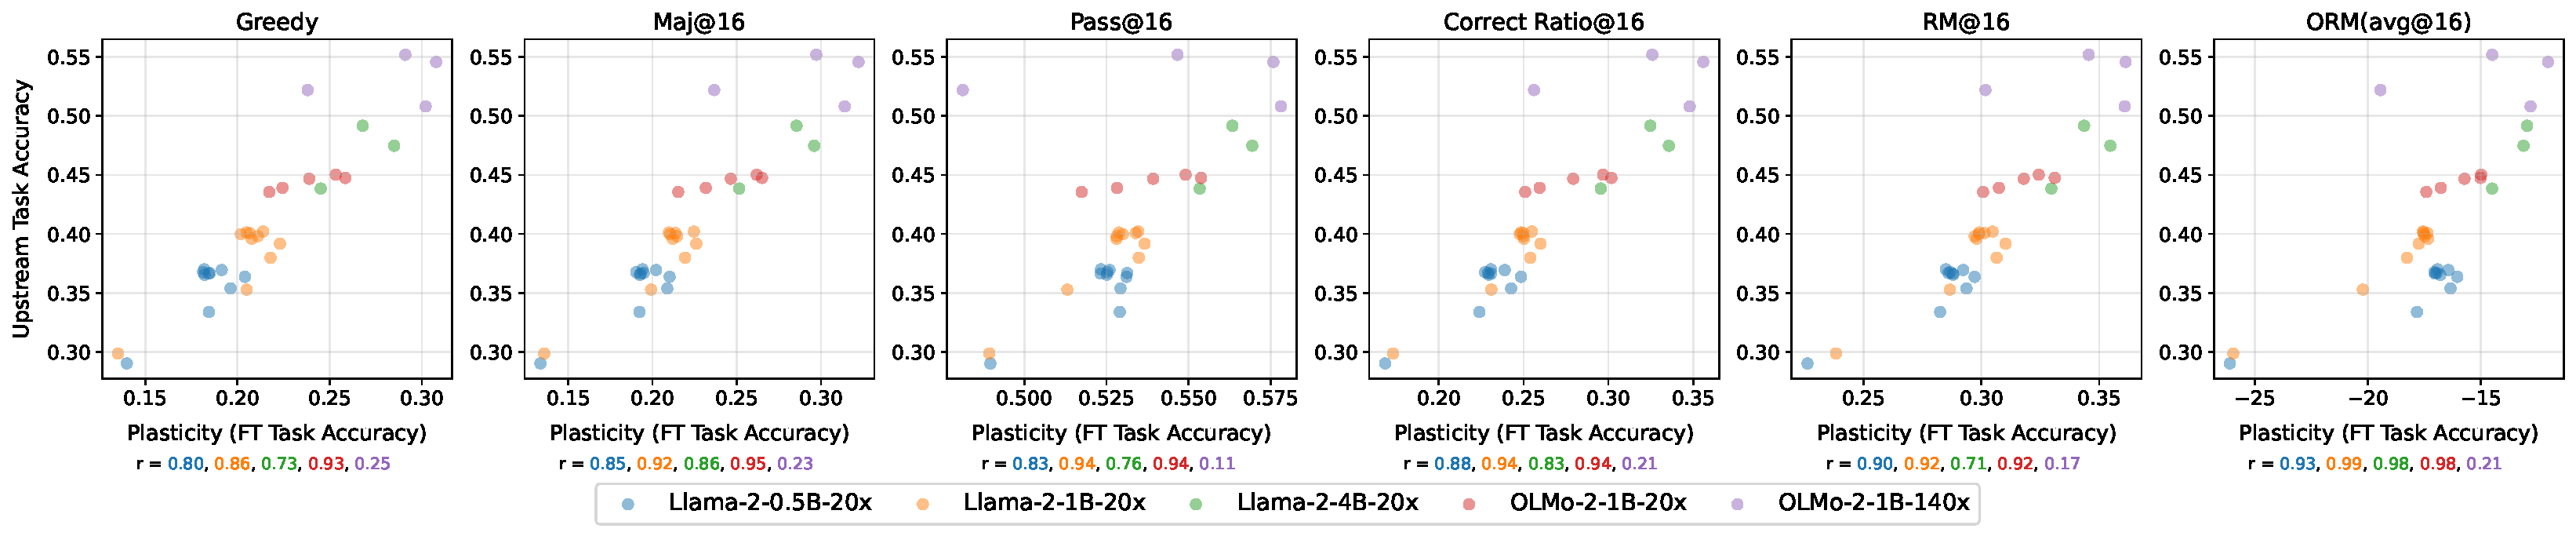
\includegraphics[width=\linewidth]{figs/a07_upstream_eval/plasticity_vs_upstream_acc.pdf}
    \caption{{\bf Plasticity vs. upstream accuracy of fine-tuned models.}} 
    \label{fig:app-plasticity-vs-upstreamacc}
\end{figure}


\begin{figure}[H] 
    \centering
        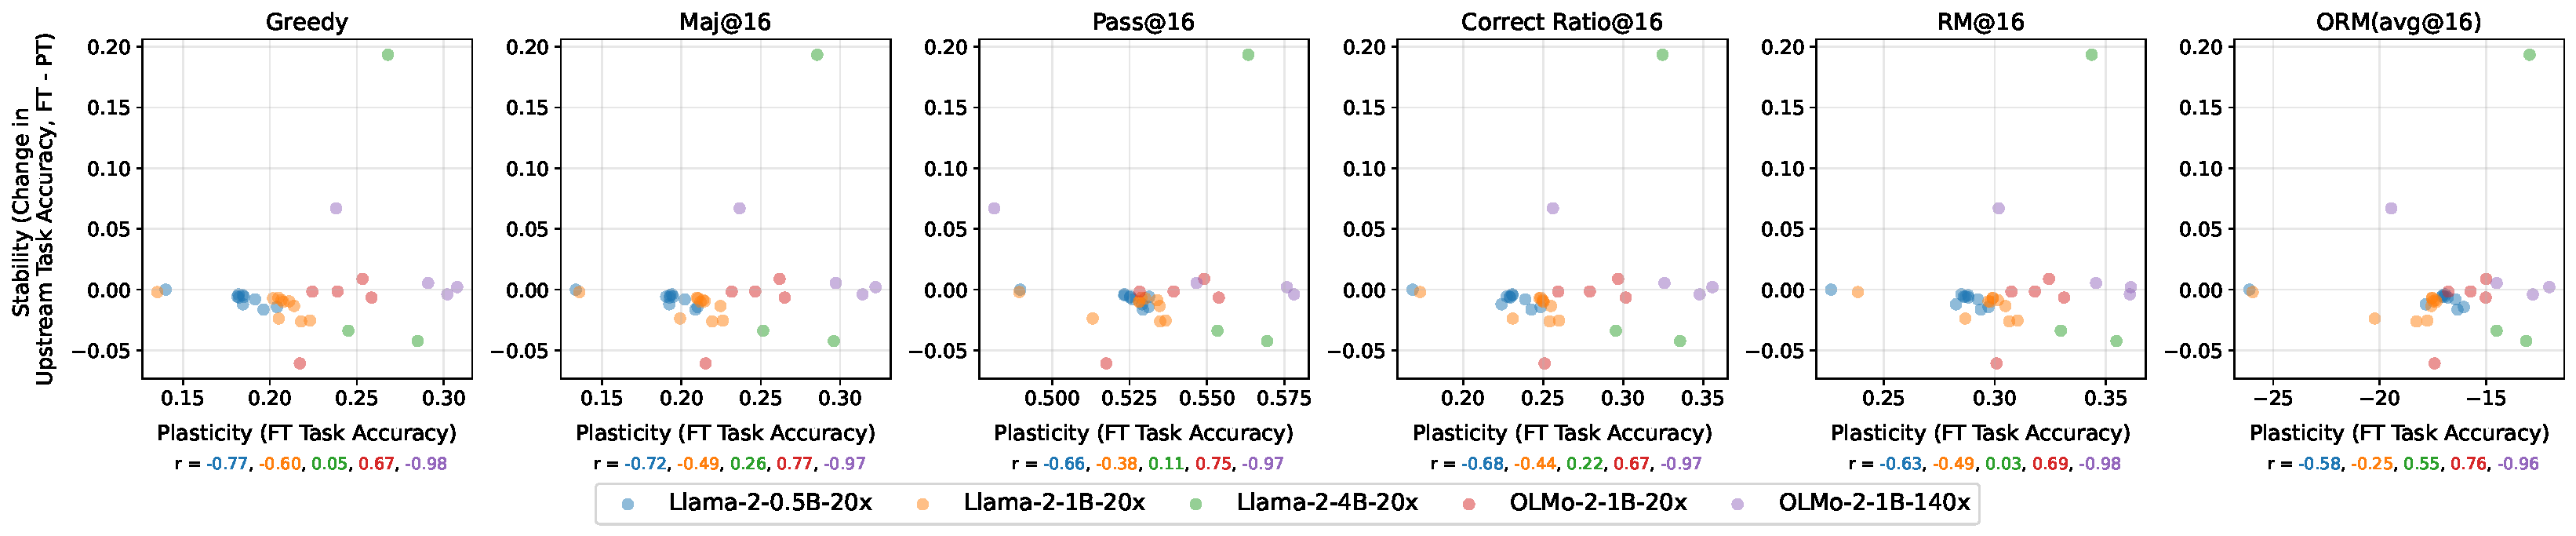
\includegraphics[width=\linewidth]{figs/a07_upstream_eval/plasticity_vs_stability.pdf}
    \caption{{\bf Plasticity vs. stability.}} 
    \label{fig:app-plasticity-vs-stability}
\end{figure}

\textbf{Can weight decay hurt upstream performance while improving downstream performance? }

To study this question, we evaluate the upstream performance of the pretrained models using the five language understanding and commonsense reasoning benchmarks. The average upstream accuracies for each model are as follows.

\llamazeropointfiveB{}, weight decay = \{0.1, 0.5, 1.0\}, upstream accuracy = \{0.40, 0.41, 0.41*\}

\llamaoneB{}, weight decay = \{0.1, 0.5, 1.0\}, upstream accuracy = \{0.44, 0.45, 0.45*\}

\olmoonex{}, weight decay = \{0.1, 0.3, 1.0\}, upstream accuracy = \{0.49, 0.49, 0.50*\}

\olmosevenx{}, weight decay = \{0.1, 0.3*, 1.0\}, upstream accuracy = \{0.61, 0.60*, 0.56\}

*weight decay value of pretrained model with best downstream performance

We find that while weight decay can lead to more plastic pretrained models that have higher performance on downstream tasks, it does not seem to affect the upstream performance of the pretrained models. 